\begin{figure}[H]
\centering
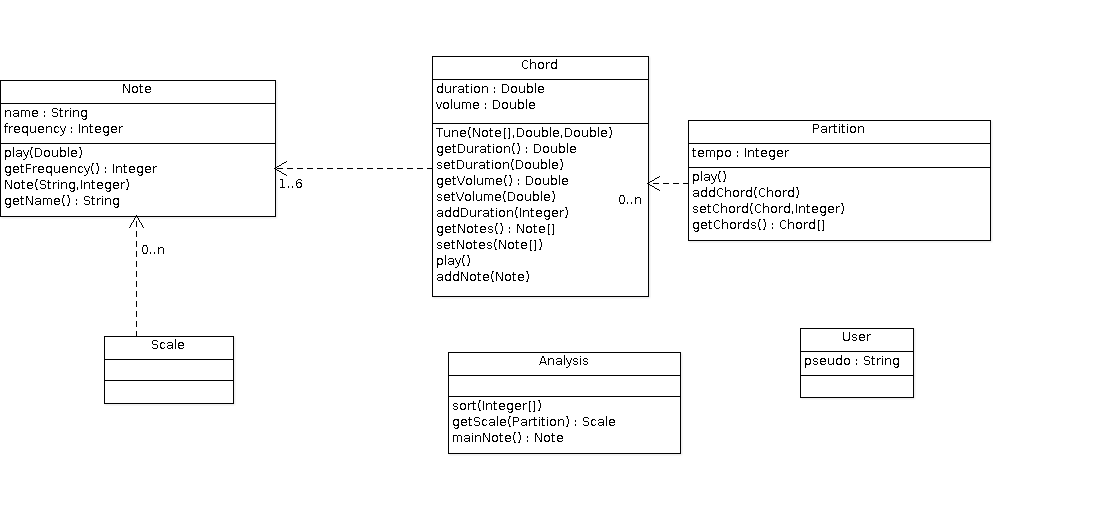
\includegraphics[scale=0.5]{ModelUML}
\caption{UML du modele}
\end{figure}

La classe Note représente une Note qui n'est pas jouée, c'est-à-dire qu'elle contient la définition d'une note seulement.\newline
La classe Chord permet donc de représenter de 1 à 6 note jouée simultanément tel un accord à la guitare.\newline
La classe Partition représente donc une partition comme l'utilisateur va la voir.\newline
La classe Analysis propose différentes fonctions essentielles à l'application. Cette classe propose également des fonctionnalités pour l'apprentissage de la composition de musiques.\newline
La classe Scale représente une gamme. Une gamme est une suite de notes, et la classe est donc composée d'un certain nombre de note.
La classe User est présente pour enregistrer le pseudonyme de l'utilisateur pour pouvoir envoyer des partitions sur le site.
Lorsque l'utilisateur va jouer une note, le logiciel va récupérer toutes les fréquences entrant par le micro et les trier en fonction de leur volume. Il est donc aisé par la suite de trouver quelles sont les notes qui sont le plus jouées.
